\cleardoublepage

\chapter{Resultados}
\label{makereference7}

Después de realizar la exploración de los parámetros de los distintos algoritmos de predicción explicados anteriormente (capítulo \ref{makereference5}), hemos obtenido varias métricas de cada uno de ellos.

\begin{itemize}
	\item Media
	\item Desviación estándar
\end{itemize}

Estas dos variables son las que nos dan la información necesaria para decantarnos por un modelo u otro. Buscamos aquella configuración de los parámetros que maximice la media y minimice el error.

La primera prueba que se realizó fue con algoritmos de regresión lineal y SVR.

De todos los resultados obtenidos, el que mayor media proporciona es un modelo realizado con Regresión Lineal, que obtiene una media de 0.910009 y un error de 0.003789. Su configuración es la siguiente:

\begin{itemize}
	\item k: 5
	\item distancia: 2
	\item copy\_X: ``true''
	\item fit\_intercept: ``true''
\end{itemize}

Esta media no es suficiente para afirmar que el modelo predictivo funciona. Para ello necesitaríamos una media mayor. Intuitivamente, una regresión lineal nunca sería capaz de proporcionarnos una buena predicción, ya que nuestros datos no son lineales. Ver figura \ref{modelo_verano}.

La segunda prueba se realizó con redes neuronales. Como este algoritmo es un clasificador ha sido necesario ``mapear'' las predicciones en distintas clases. Debido a que estos datos han sido normalizados, es sencillo clasificarlos en 100 clases [0, 100]. La intención de estas clases no es tanto acertar la cantidad de radiación sino proporcionar un rango en la que se encontrará.

\begin{figure}[htb]
	\begin{center}
		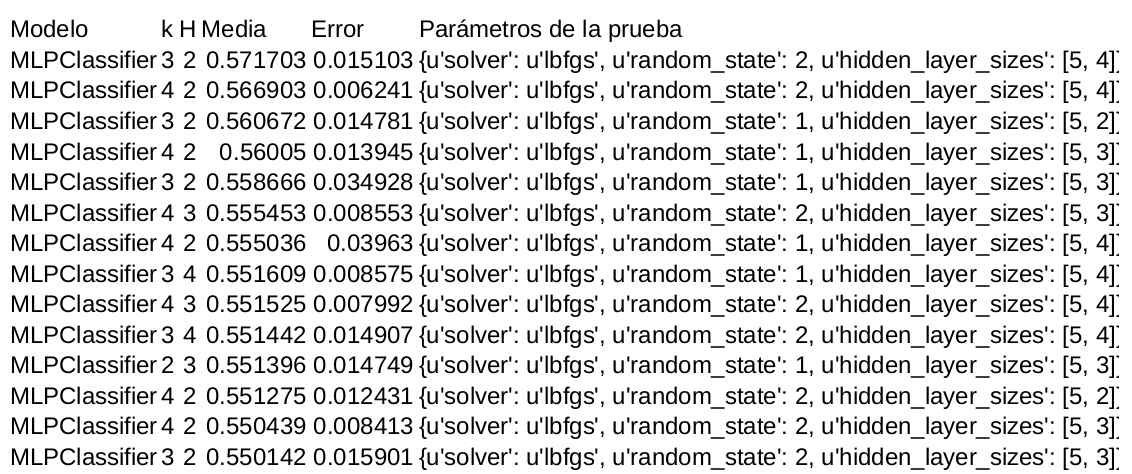
\includegraphics[width=14cm]{figures/resultado_mlp.png}
		\caption{Resultado redes neuronales \label{resultado_mlp}}
	\end{center}
\end{figure}

Una vez realizadas las pruebas, se observa que la media es muy baja,0.539901 en el mejor caso. Descartamos utilizar estos modelos de redes neuronales en nuestro proyecto.

Como futura vía de estudio se plantea volver a realizar este entrenamiento replanteando los parámetros y el ``mapeo'' de las clases.

Finalmente, hemos elegido el modelo SVR con las configuraciones siguientes:

\begin{itemize}
	\item k: 4
	\item distancia: 2
	\item kernel: ``rbf''
	\item C: 1000
	\item gamma: 0.001
\end{itemize}

\begin{figure}[htb]
	\begin{center}
		\includegraphics[width=16cm]{figures/resultado_elegido.png}
		\caption{Resultado elegido \label{resultado_elegido}}
	\end{center}
\end{figure}

Aunque no es el modelo con más media ni menos error, es de los más equilibrados. Esta configuración obtiene una media de acierto de 0.901516, distanciándose en 0.008493 de la media máxima conseguida. Su error es de 0.000330. Además se intuye que SVR debería ser el modelo que mejor se ajuste. Por lo que en un futuro estudio que busque mejorar esta predicción, sería un buen punto de partida.

\section{Calidad del código}
\label{makereference7.1}

Una vez acabado el código del proyecto, decidimos certificar su calidad mediante \href{https://www.codacy.com}{Codacy}.
Codacy es una herramienta que proporciona nuestro controlador de versiones GitHub. Sencillamente revisa todas y cada una de las líneas del código, para hacerlo más sencillo, escalable y seguro. Genera un informe con los errores y te dice qué grado de calidad tiene, siendo A el más alto. (\cite{ARP:Codacy:2017})

\begin{figure}[htb]
	\begin{center}
		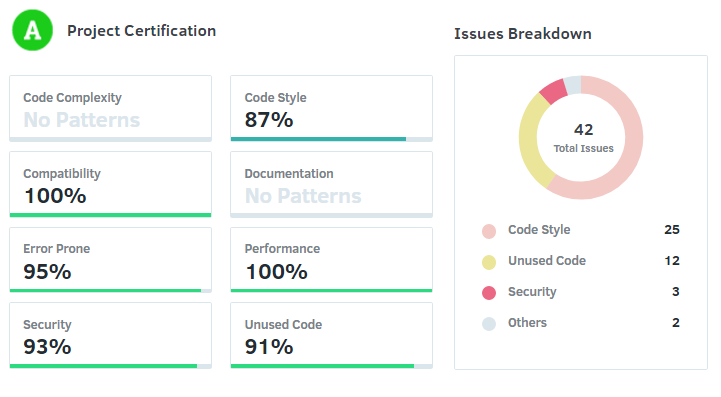
\includegraphics[height=3.5in]{figures/codacy.png}
		\caption{Informe de nuestro proyecto [Fuente: \href{https://www.codacy.com}{Codacy}] \label{codacy}}
	\end{center}
\end{figure}